\subsection{M-array Pattern Projection Method \cite{morita1988reconstruction}}

The binary M-array pattern projection method consists in projecting dark and light dots. The color of each dot represent a 0 (dark) or 1 (light) of the M-array pattern. The spatial coordinates of each dot matched with a projected one of the pattern can be determined by triangulation. However, pattern disorders occur often in the observed pattern. One of the asset of this method is the detection and correction of pattern disorders.

\subsubsection{Pattern Disorders}

There are three different types of pattern disorder.
\begin{itemize}
\item Deficiency of dots. If there are several object in the scene, an object may obstruct the pattern. On the Figure \ref{fig:disorder1}, the first second and third dots are not visible by the camera.
\item Displacement due to Difference in Depth : in comparison to the initial pattern projected, the dots may shift because of the depth of each object. On the Figure \ref{fig:disorder1}, the dots 4 to 5 on the object 2 have shifted compared with the dots of object 1.
\item Permutation of dots : if an object is in front of another, the order of dots may change. On the Figure \ref{fig:disorder1}, the dot 3 has changed of order and is the fourth one from the point of view of the camera.
\end{itemize}

\begin{figure}[h]
  %\centering
  \centerline{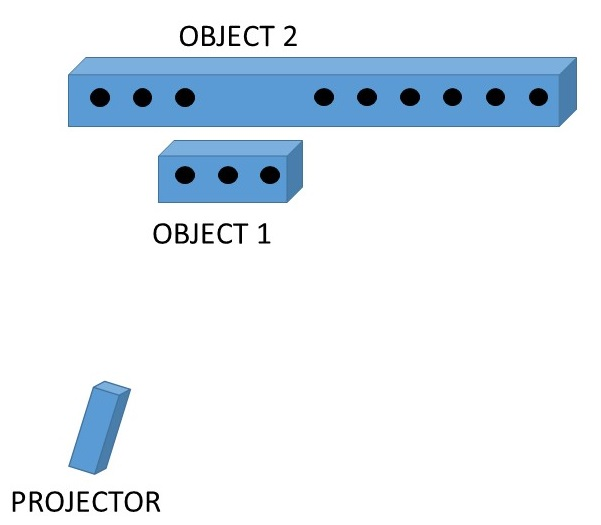
\includegraphics[scale=0.6]{fig/disorder1.jpg}}
  \caption{Pattern Disorders}
  \label{fig:disorder1}
\end{figure}






\subsubsection{Correction of Pattern Disorders}
There are four steps in the matching of the observed dots with those of the pattern and the correction of the pattern disorders.





\paragraph{Temporary Array}
The image recorded is analyzed line per line of dots and a 2-D array which contains the numbers of the observed dots is created. The array can be computed by these steps :
\begin{itemize}
\item Creation of the array (all the elements are set to zero).
\item Scan of the image to detect dots. Each time a dot is found, its value and position are saved into 1-D arrays VALUE, X and Y.
\item The position of the dots are quantized using X and Y so that adjoining dots have consecutive quantized coordinates.
\item Insertion of the number of each dot into the array (the location into the array corresponds to the quantized coordinates).
\end{itemize}

This temporary array (T-array) may has some vacant places due to disorder pattern.

\paragraph{Grow}
Each element of the T-array gets an index (column number of the M-array). To do so, a window is defined and applied to the T-array and the M-array where the elements into the window of each array have the same value. The element into the window of the T-array can be indexed using the M-array and the two windows moved simultaneously by one column or row. This is repeated until a difference between the two windows is detected. New windows are then initialized elsewhere. The grow terminate when no window can be initialized to an area of the T-array where there is no index yet.


\paragraph{Detection of pattern disorders}




